\documentclass[tikz,border=12pt]{standalone}
% Shared visual language for standalone EMT block diagrams.
\usepackage{amsmath}
\usetikzlibrary{arrows.meta,backgrounds,calc,fit,positioning}

\tikzset{
    emt diagram/.style = {>={Stealth[length=2.4mm]}},
    line/.style        = {semithick, rounded corners=6pt},
    block/.style       = {draw, semithick, fill=white,
                          minimum height=1cm, minimum width=2.3cm},
    hblock/.style      = {block, minimum width=2.24cm, minimum height=1.3cm},
    vblock/.style      = {block, minimum width=1.3cm, minimum height=2.24cm},
    sum/.style         = {draw, semithick, fill=white, circle,
                          inner sep=2.6pt},
    signal/.style      = {circle, fill, inner sep=1.4pt,
                          label distance=3pt},
    sig/.style         = {font=\small},
    pm/.style          = {font=\scriptsize},
    wire jump/.style   = {line,
                          preaction={draw=white, line width=3pt,
                                     line cap=round}},
    enclosure/.style   = {draw, dashed, semithick, rounded corners=4pt},
    operator enclosure/.style = {enclosure, inner xsep=7mm, inner ysep=6mm}
}

% Scalar control symbols shared by the REECB and REPCA figures.
% Static saturation characteristics and non-windup limits on dynamic blocks.
% The model READMEs define smooth realizations and state-enable gates.
\newcommand{\staticlimit}[4]{%
    \node[minimum width=1.1cm, minimum height=1cm, inner sep=0pt]
        (#1) at #2 {};
    \draw[semithick] (#1.west) -- (#1.east);
    \draw[semithick] ($(#1.center)+(-0.43,-0.4)$)
        -- ++(0.28,0) -- ++(0.3,0.8) -- ++(0.28,0);
    \node[sig, above=1pt of #1] {$#4$};
    \node[sig, below=1pt of #1] {$#3$};
}
\newcommand{\nonwindup}[3]{%
    \draw[semithick] (#1.north) -- ++(0.12,0.26) -- ++(0.3,0)
        node[sig, above] {$#3$};
    \draw[semithick] (#1.south) -- ++(-0.12,-0.26) -- ++(-0.3,0)
        node[sig, below] {$#2$};
}
\newcommand{\deadbandblock}[4]{%
    \node[block, minimum width=1.4cm, minimum height=1.15cm]
        (#1) at #2 {};
    \draw[thin] ($(#1.center)+(-0.53,0)$) -- ++(1.06,0);
    \draw[thin] ($(#1.center)+(0,-0.43)$) -- ++(0,0.86);
    \draw[semithick] ($(#1.center)+(-0.45,-0.38)$)
        -- ++(0.27,0.38) -- ++(0.36,0) -- ++(0.27,0.38);
    \node[sig, above=2pt of #1] {$#3,\,#4$};
}
% Inputs are -one (upper) and -zero (lower); output is -out.
\newcommand{\controlselector}[3]{%
    \coordinate (#1-one) at ($#2+(-0.4,0.4)$);
    \coordinate (#1-zero) at ($#2+(-0.4,-0.4)$);
    \coordinate (#1-out) at ($#2+(0.45,0)$);
    \fill (#1-one) circle (1.4pt);
    \fill (#1-zero) circle (1.4pt);
    \draw[semithick] (#1-out) -- ($#2+(-0.26,0.32)$);
    \node[pm, right=3pt] at (#1-one) {$1$};
    \node[pm, right=3pt] at (#1-zero) {$0$};
    \node[sig, above=15pt] at #2 {$#3$};
}


% TUNABLES: reactive-command, active-command, and frequency-response rows.
\def\reactiverow{1.6}
\def\activerow{-3.6}
\def\frequencyrow{-7.2}

\begin{document}
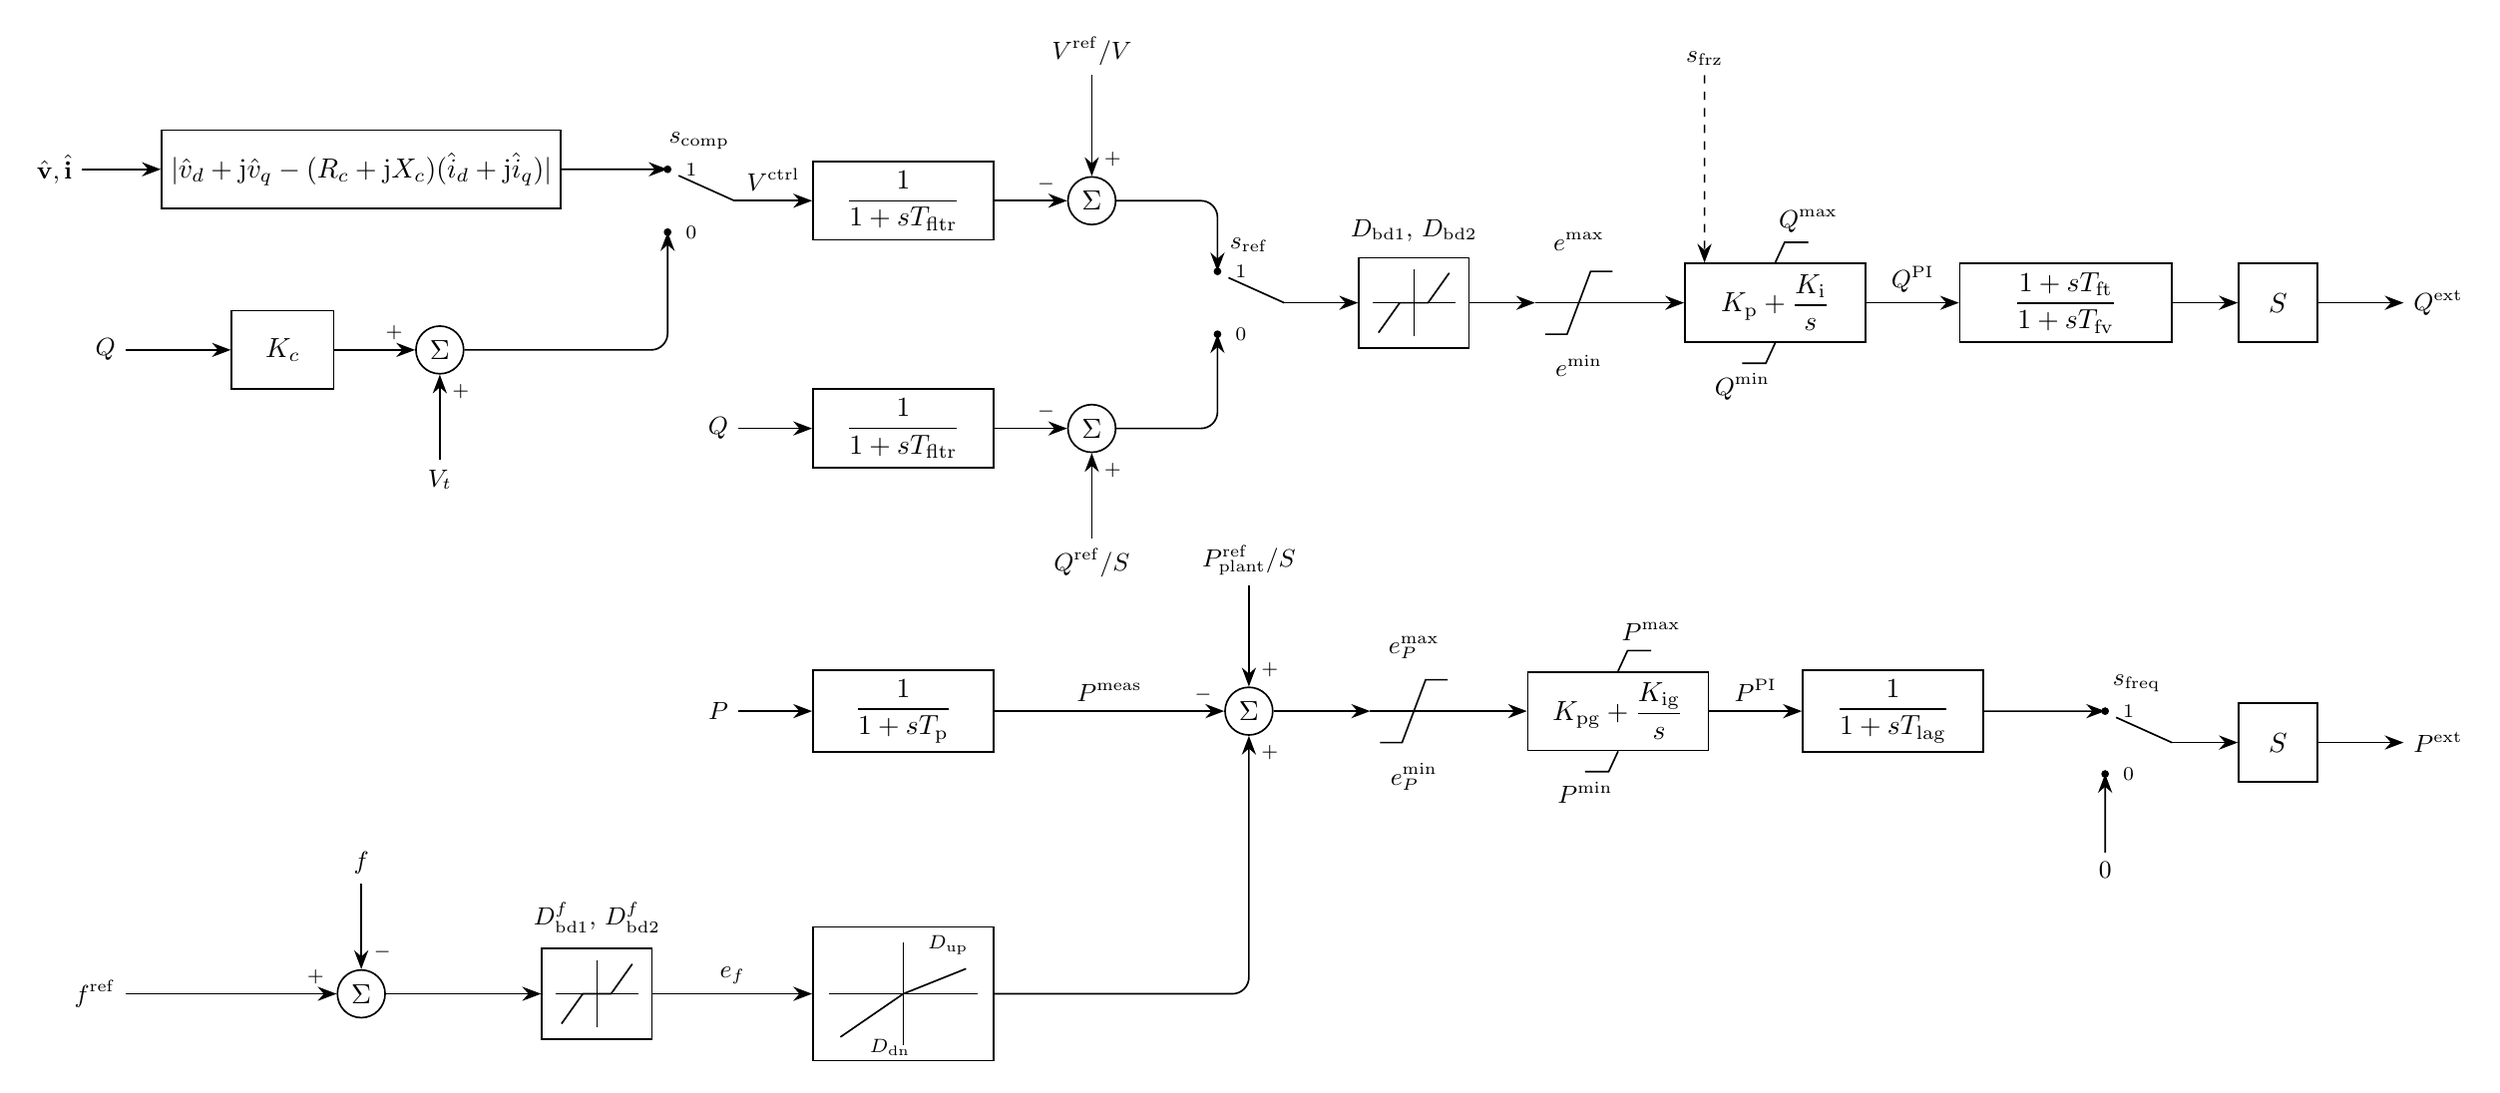
\begin{tikzpicture}[emt diagram, block/.append style={align=center}]

% Compensated voltage and independently filtered voltage / reactive power.
\node[block,minimum width=3.7cm] (ldc) at (0,3.3)
    {$|\hat v_d+\mathrm j\hat v_q-(R_c+\mathrm jX_c)(\hat i_d+\mathrm j\hat i_q)|$};
\draw[->,line] ([xshift=-1cm]ldc.west) node[sig,left] {$\hat{\mathbf v},\hat{\mathbf i}$} -- (ldc.west);
\node[block,minimum width=1.3cm] (kc) at (-1,1) {$K_c$};
\draw[->,line] (-3,1) node[sig,left] {$Q$} -- (kc.west);
\node[sum] (droopv) at (1,1) {$\Sigma$};
\draw[->,line] (kc.east) -- (droopv.west);
\node[pm,above left=0pt and 1pt of droopv.west] {$+$};
\draw[->,line] (1,-0.4) node[sig,below] {$V_t$} -- (droopv.south);
\node[pm,below right=0pt and 1pt of droopv.south] {$+$};
\controlselector{comp}{(4.3,2.9)}{s_{\mathrm{comp}}}
\draw[->,line] (ldc.east) -- (comp-one);
\draw[->,line] (droopv.east) -| (comp-zero);
\node[block] (vlag) at (6.9,2.9) {$\dfrac{1}{1+sT_{\mathrm{fltr}}}$};
\draw[->,line] (comp-out) -- node[sig,above] {$V^{\mathrm{ctrl}}$} (vlag.west);
\node[sum] (ev) at (9.3,2.9) {$\Sigma$};
\draw[->,line] (vlag.east) -- (ev.west);
\node[pm,above left=0pt and 1pt of ev.west] {$-$};
\draw[->,line] (9.3,4.5) node[sig,above] {$V^{\mathrm{ref}}/V$} -- (ev.north);
\node[pm,above right=0pt and 1pt of ev.north] {$+$};
\node[block] (qlag) at (6.9,0) {$\dfrac{1}{1+sT_{\mathrm{fltr}}}$};
\draw[->,line] (4.8,0) node[sig,left] {$Q$} -- (qlag.west);
\node[sum] (eq) at (9.3,0) {$\Sigma$};
\draw[->,line] (qlag.east) -- (eq.west);
\node[pm,above left=0pt and 1pt of eq.west] {$-$};
\draw[->,line] (9.3,-1.4) node[sig,below] {$Q^{\mathrm{ref}}/S$} -- (eq.south);
\node[pm,below right=0pt and 1pt of eq.south] {$+$};
\controlselector{ref}{(11.3,\reactiverow)}{s_{\mathrm{ref}}}
\draw[->,line] (ev.east) -| (ref-one);
\draw[->,line] (eq.east) -| (ref-zero);
\deadbandblock{dbq}{(13.4,\reactiverow)}{D_{\mathrm{bd1}}}{D_{\mathrm{bd2}}}
\staticlimit{eqmax}{(15.5,\reactiverow)}{e^{\min}}{e^{\max}}
\node[block] (piq) at (18,\reactiverow) {$K_{\mathrm p}+\dfrac{K_{\mathrm i}}{s}$};
\nonwindup{piq}{Q^{\min}}{Q^{\max}}
\node[block,minimum width=2.7cm] (leadlag) at (21.7,\reactiverow) {$\dfrac{1+sT_{\mathrm{ft}}}{1+sT_{\mathrm{fv}}}$};
\node[block,minimum width=1cm] (qscale) at (24.4,\reactiverow) {$S$};
\draw[->,line] (ref-out) -- (dbq.west);
\draw[->,line] (dbq.east) -- (eqmax.west);
\draw[->,line] (eqmax.east) -- (piq.west);
\draw[->,line] (piq.east) -- node[sig,above] {$Q^{\mathrm{PI}}$} (leadlag.west);
\draw[->,line] (leadlag.east) -- (qscale.west);
\draw[->,line] (qscale.east) -- (26,\reactiverow) node[sig,right] {$Q^{\mathrm{ext}}$};
\draw[->,line,dashed] (17.1,4.5) node[sig,above] {$s_{\mathrm{frz}}$}
    -- ([xshift=-9mm]piq.north);

% Plant active-power feedback, error limit, and non-windup PI.
\node[block] (plag) at (6.9,\activerow) {$\dfrac{1}{1+sT_{\mathrm p}}$};
\draw[->,line] (4.8,\activerow) node[sig,left] {$P$} -- (plag.west);
\node[sum] (ep) at (11.3,\activerow) {$\Sigma$};
\draw[->,line] (plag.east) -- node[sig,above] {$P^{\mathrm{meas}}$} (ep.west);
\node[pm,above left=0pt and 1pt of ep.west] {$-$};
\draw[->,line] (11.3,-2) node[sig,above] {$P_{\mathrm{plant}}^{\mathrm{ref}}/S$} -- (ep.north);
\node[pm,above right=0pt and 1pt of ep.north] {$+$};
\staticlimit{epmax}{(13.4,\activerow)}{e_P^{\min}}{e_P^{\max}}
\node[block] (pip) at (16,\activerow) {$K_{\mathrm{pg}}+\dfrac{K_{\mathrm{ig}}}{s}$};
\nonwindup{pip}{P^{\min}}{P^{\max}}
\node[block] (lagp) at (19.5,\activerow) {$\dfrac{1}{1+sT_{\mathrm{lag}}}$};
\controlselector{freq}{(22.6,-4)}{s_{\mathrm{freq}}}
\draw[->,line] (ep.east) -- (epmax.west);
\draw[->,line] (epmax.east) -- (pip.west);
\draw[->,line] (pip.east) -- node[sig,above] {$P^{\mathrm{PI}}$} (lagp.west);
\draw[->,line] (lagp.east) -- (freq-one);
\draw[->,line] (22.2,-5.4) node[sig,below] {$0$} -- (freq-zero);
\node[block,minimum width=1cm] (pscale) at (24.4,-4) {$S$};
\draw[->,line] (freq-out) -- (pscale.west);
\draw[->,line] (pscale.east) -- (26,-4) node[sig,right] {$P^{\mathrm{ext}}$};

% Asymmetric frequency droop, drawn as its input-output characteristic.
\node[sum] (ef) at (0,\frequencyrow) {$\Sigma$};
\draw[->,line] (-3,\frequencyrow) node[sig,left] {$f^{\mathrm{ref}}$} -- (ef.west);
\node[pm,above left=0pt and 1pt of ef.west] {$+$};
\draw[->,line] (0,-5.8) node[sig,above] {$f$} -- (ef.north);
\node[pm,above right=0pt and 1pt of ef.north] {$-$};
\deadbandblock{dbf}{(3,\frequencyrow)}{D_{\mathrm{bd1}}^f}{D_{\mathrm{bd2}}^f}
\node[block,minimum width=2.3cm,minimum height=1.7cm] (df) at (6.9,\frequencyrow) {};
\draw[thin] ($(df.center)+(-0.95,0)$) -- ++(1.9,0);
\draw[thin] ($(df.center)+(0,-0.65)$) -- ++(0,1.3);
\draw[semithick] ($(df.center)+(-0.8,-0.55)$) -- (df.center) -- ++(0.8,0.32);
\node[pm,anchor=north west] at ($(df.center)+(-0.55,-0.46)$) {$D_{\mathrm{dn}}$};
\node[pm,anchor=south east] at ($(df.center)+(0.95,0.38)$) {$D_{\mathrm{up}}$};
\draw[->,line] (ef.east) -- (dbf.west);
\draw[->,line] (dbf.east) -- node[sig,above] {$e_f$} (df.west);
\draw[->,line] (df.east) -| (ep.south);
\node[pm,below right=0pt and 1pt of ep.south] {$+$};

\end{tikzpicture}
\end{document}
